\documentclass[../notes.tex]{subfiles}

\pagestyle{main}
\renewcommand{\chaptermark}[1]{\markboth{\chaptername\ \thechapter\ (#1)}{}}
\setcounter{chapter}{2}

\begin{document}




\chapter{Proteins}
\section{Amino Acids, Peptides, and Protein Synthesis}
\begin{itemize}
    \item \marginnote{10/11:}Initial impressions of the homework: More difficult than expected.
    \begin{itemize}
        \item Tang did not raise the difficulty of the course, but was told to in course evals two years ago.
        \item Literature problems: People believe reading the papers did help with the questions. We should be able to do these problems without the papers, though --- some of these problems are past exam problems and were expected to be answered in a closed-book setting. We can expect similar questions on exams this year. Purpose: Show us how concepts from the class are used in research.
    \end{itemize}
    \item There will be a practice exam posted.
    \item We can bring a one-page (single-sided A4) review sheet to the exam.
    \item OH Monday via Zoom.
    \item For every Thursday midterm, the content from the preceding Tuesday will not be covered.
    \item \textbf{Lesion}: Something bad that your cell will recognize and repair.
    \item Types of lesions:
    \begin{itemize}
        \item Double-stranded breaks, mismatches, pyrimidine dimers, and damaged bases.
        \item Are mutations lesions? It depends.
        \begin{itemize}
            \item If the mutation is a mismatch, there will be a repair.
            \item If it shows up as matched, your cell will not know to repair it.
        \end{itemize}
        \item DNA modifications.
        \begin{itemize}
            \item Damaged backbones (e.g., pyrimidine dimers or a methyl group on the $O^6$ of guanine). Things your cells know shouldn't be there. Will be repaired.
            \item However, there can also be intentionally placed modifications on DNA to regulate it. These will not be repaired.
        \end{itemize}
        \item Bulges don't usually occur during synthesis, but they can occur during recombination. These will definitely be repaired.
        \item This should clarify some points on the homework.
    \end{itemize}
    \item Natural base modification in mRNA.
    \begin{itemize}
        \item mRNA is less diversely modified than tRNA and rRNA, but mRNA modifications do still happen.
        \item Most abundant internal modifications in mammalian mRNA: $N^6$-methyladenosine (\ce{m^6A}).
        \begin{itemize}
            \item There's on average 1-3 of these per mRNA. However, there can still be 0.
            \item How it's detected: Highly related to ChIP-Seq. You fragment your DNA, introduce antibodies that will bind to \ce{m^6A}, do immunoprecipitation for a specific DNA binding protein to enrich the target DNA sequence, and sequence both the input and the enriched pool. The sequences that got enriched are the ones that carry the modification.
        \end{itemize}
        \item 5-methylcytosine (\ce{m^5C}) and pseudouridine ($\psi$) are also present in mRNA, but their functions are less well studied.
        \begin{itemize}
            \item Pseudouridine is a flipped uracil base with a carbon connected to ribose instead of a nitrogen connected to ribose.
            \item The W-C interaction surface is basically unchanged, though, so it will still be detected as U. However, it has alternate regulatory functions, such as helping ribosomes read through premature stop codons.
            \item The $\psi$ detection method is messy (noisy): Introduce a chemical that selectively reacts with pseudouridine and gives a stop-signal during transcription. Not testable.
            \item 5mC detection for RNA is identical to for DNA (bisulfite chemistry --- see the discussion associated with Figure \ref{fig:bisulfite}). Note, however, that since RNA is less stable, more will decompose upon heating; thus, you need a larger initial sample size.
        \end{itemize}
        \item In addition to \ce{m^6A}, \ce{m^5C}, and $\psi$, other base modifications can occur (we are not responsible for these, though).
    \end{itemize}
    \item Summary of what we've learned so far:
    \begin{itemize}
        \item DNA synthesis and transcription (the $\text{DNA}\to\text{RNA}$ part of the central dogma).
        \item DNA methylation and epigenetics.
        \item mRNA methylation and epitranscriptomics.
        \item These three things function as a network (many feedback mechanisms). Moving forward, we will add proteins and metabolites to this network.
    \end{itemize}
    \item Not testable: Arms race between bacteria and bacteriophages.
    \begin{itemize}
        \item Answers how weird DNA modifications develop.
        \item Bacteriophages are the most abundant life organism on this earth.
        \item Round 1: Bacteria evolve restriction enzymes and base modification X; purpose: cleave phage DNA while avoiding suicide.
        \item Round 2: Phages evolve X or Y modification in DNA; purpose: escape cleavage.
        \item Round 3: Bacteria evolve X/Y-dependent restriction enzymes and additional self base modification Z; purpose: cleave phage DNA while avoiding suicide.
        \item And on and on.
    \end{itemize}
    \item Diverse base modifications in bacteriophages.
    \begin{itemize}
        \item Guanine converts $N^7$ to a carbon and adds a functional group; you need multiple modifications to get to this result (called deoxyarchaeosine).
        \item Cytosine attaches to glucose instead of deoxyribose.
        \item Some bacteriophage DNA/RNA base modifications overlap with those in higher organisms, who evolve these modifications for completely different reasons.
        \item And more.
    \end{itemize}
    \item We are now done with last lecture's content; we are moving onto amino acids, peptides, and proteins.
    \begin{itemize}
        \item Note that many of the mechanisms of RNA are more complicated than those of proteins, so if you have trouble with the latter, review the former.
        \item Primarily amino acids this lecture; peptides, proteins, and higher-order structures next lecture.
        \item Hopefully, these first six lectures will be foundational for the week 5-7 lectures on organelles and cell biology.
    \end{itemize}
    \item A chemical look at proteins.
    \begin{itemize}
        \item Made of proteinogenic amino acids (natural L-amino acids save glycine).
        \item Can be post-translationally modified.
        \item Post-translational rearrangement (lecture on this later).
        \item We will look at amino acid properties.
        \item Next lecture: Determinants of protein structure and\dots
        \item Secondary and higher order structures.
    \end{itemize}
    \item \textbf{Protein}: A polymer composed of amino acids.
    \begin{itemize}
        \item Grows from the N-terminus to the C-terminus.
    \end{itemize}
    \item Chirality is key.
    \begin{itemize}
        \item Except for the achiral glycine, (almost) every amino acid is in its L-form.
        \begin{itemize}
            \item Amino acids in their D-form are used as monomers, not for protein synthesis.
        \end{itemize}
        \item Steve Kent synthesized the D-form of HIV protease; he's a giant in the field. Taught here.
        \begin{itemize}
            \item His big contribution is the development of \textbf{native chemical ligation}, while he was at Scripps.
            \item We will talk about this more when we cover bioorthogonal chemistry.
        \end{itemize}
        \item No ribosomal D-protein synthesis because we would need an entire mirror image biological system.
        \begin{itemize}
            \item People are trying to build a mirror ribosome, which Tang thinks is crazy, but they are making progress.
        \end{itemize}
        \item Total protein synthesis hasn't gone beyond 300 amino acids.
        \begin{itemize}
            \item Solid state protein synthesis: Add one amino acid at a time. Highly efficient. $99.5\%$ efficiency is great, but we have an exponential decrease of yield. Thus, we can't synthesize more than 50-100 amino acid peptides at a time.
            \item Strategy: Fragments of 50 amino acids ligated together with natural chemical ligation.
            \item But since proteins are folded as they're built in real life, we natural chemical ligation doesn't necessarily result in an accurately folded protein.
        \end{itemize}
    \end{itemize}
    \item \textbf{Native chemical ligation}: Connecting two peptides with an amide bond.
    \begin{itemize}
        \item A very hard chemical problem; requires activating the amine of an amino acid.
    \end{itemize}
    \item Taking advantage of D-proteins.
    \begin{itemize}
        \item Why we want to do this: To challenge nature. Tang thinks this is stupid, though.
        \item Favorable features of D peptides/proteins.
        \begin{itemize}
            \item Similar to L proteins: bind to DNA/RNA/proteins, can catalyze reactions.
            \item Cannot be degraded by natural protease (much more stable than natural peptides/proteins).
        \end{itemize}
        \item Challenges in identifying D peptides/proteins that bind specifically to a natural protein.
        \begin{itemize}
            \item Rational design? --- Hard to do with so many variables.
            \item Screening? --- Synthesize a D peptide library that can be amplified between selection rounds.
        \end{itemize}
        \item You can't synthesize a D library to look for hits on an L target (too hard; no mirror ribosomes). So instead, synthesize an L library, look for a hit on a D target, and then synthesize the D version of your L hit, which (flipping both chiralities) will react with your L target.
        \begin{itemize}
            \item A brilliant idea but didn't turn out that well, though.
        \end{itemize}
        \item D-proteins aren't as big as they might be because there are many ways proteins can be degraded \emph{in vivo} (not just natural proteases).
    \end{itemize}
    \item Protein basics.
    \begin{itemize}
        \item Classification of amino acids is somewhat arbitrary, but they are loosely categorized into hydrophobic, charged, polar, and glycine (in a class by itself since it's achiral).
        \begin{itemize}
            \item For example, tryptophan could conceivably be hydrophobic or polar.
            \item Histidine can frequently be charged.
            \item Knowing properties is more important than knowing classes.
        \end{itemize}
        \item Knowing the amino acids is essential for predicting things like how amino acids interact with each other, what their role is in a reaction, how they catalyze a reaction, etc.
        \item Memorize amino acids!
        \begin{itemize}
            \item The 3-letter and 1-letter shorthand is often (but not always) the first 3 (resp. 1) letter(s) of the name.
        \end{itemize}
    \end{itemize}
    \item Achiral amino acid.
    \begin{figure}[h!]
        \centering
        \footnotesize
        \begin{subfigure}[b]{0.19\linewidth}
            \centering
            \chemfig{H_2N-[:30](-[:70]H)(-[:110]H)-[:-30]COOH}
            \caption{Glycine.}
            \label{fig:AAachiralG}
        \end{subfigure}
        \caption{Achiral amino acid.}
        \label{fig:AAachiral}
    \end{figure}
    \begin{itemize}
        \item Glycine.
        \begin{itemize}
            \item Flexible since it's unsubstituted on its $\alpha$-carbon; can sample multiple conformations.
            \item Whenever you have a glycine in your protein, you can assume the protein is flexible in that region.
            \item If you want to fuse two proteins together but you're worried about sterics, you typically use a GGS (glycine, glycine, serine) linker.
            \item Name: Glycine, Gly, G.
        \end{itemize}
    \end{itemize}
    \item Hydrophobic amino acids.
    \begin{figure}[H]
        \centering
        \footnotesize
        \begin{subfigure}[b]{0.16\linewidth}
            \centering
            \chemfig{H_2N-[:30](<[2])-[:-30]COOH}
            \caption{Alanine.}
            \label{fig:AAachiralA}
        \end{subfigure}
        \begin{subfigure}[b]{0.16\linewidth}
            \centering
            \chemfig{H_2N-[:30](<[2](-[::60])(-[::-60]))-[:-30]COOH}
            \caption{Valine.}
            \label{fig:AAachiralV}
        \end{subfigure}
        \begin{subfigure}[b]{0.16\linewidth}
            \centering
            \chemfig{H_2N-[:30](<[2]-[::-60](-[::60])(-[::-60]))-[:-30]COOH}
            \caption{Leucine.}
            \label{fig:AAachiralL}
        \end{subfigure}
        \begin{subfigure}[b]{0.16\linewidth}
            \centering
            \chemfig{H_2N>[:30](-[2](<[::60])(-[::-60]-[::60]))-[:-30]COOH}
            \caption{Isoleucine.}
            \label{fig:AAachiralI}
        \end{subfigure}
        \begin{subfigure}[b]{0.16\linewidth}
            \centering
            \chemfig{H_2N-[:30](<[2]-[::-60]-[::60]S-[::60])-[:-30]COOH}
            \caption{Methionine.}
            \label{fig:AAachiralM}
        \end{subfigure}
        \begin{subfigure}[b]{0.16\linewidth}
            \centering
            \chemfig{[:-24]*5(-[,,,2]HN-(-COOH)<--)}
            \caption{Proline.}
            \label{fig:AAachiralP}
        \end{subfigure}\\[2em]
        \begin{subfigure}[b]{0.25\linewidth}
            \centering
            \chemfig{H_2N-[:30](<[2](-[:150,,,,white]-[:-150,,,,white]-[:150,,,,white])-[:30]*6(=-=-=-))-[:-30]COOH}
            \caption{Phenylalanine.}
            \label{fig:AAachiralF}
        \end{subfigure}
        \begin{subfigure}[b]{0.3\linewidth}
            \centering
            \chemfig{H_2N-[:30](<[2](-[:150,,,,white]-[:-150,,,,white]-[:150,,,,white]-[:150,,,,white]\phantom{HO})-[:30]*6(=-=(-OH)-=-))-[:-30]COOH}
            \caption{Tyrosine.}
            \label{fig:AAachiralT}
        \end{subfigure}
        \begin{subfigure}[b]{0.25\linewidth}
            \centering
            \chemfig{H_2N-[:30](<[2](-[:135,,,,white]-[:162,,,,white]-[:-150,,,,white]-[:150,,,,white])-[:45]*5([::27]-*6(-=-=-=)-[,,,,opacity=0]-\chemabove{N}{H}-=))-[:-30]COOH}
            \caption{Tryptophan.}
            \label{fig:AAachiralW}
        \end{subfigure}
        \caption{Hydrophobic amino acids.}
        \label{fig:AAhydrophobic}
    \end{figure}
    \begin{itemize}
        \item We start with the \emph{aliphatic} hydrophobic amino acids.
        \item Alanine.
        \begin{itemize}
            \item Simplest chiral amino acid. That's what makes it important. No other important features.
            \item If you think an amino acid is important, mutate it to alanine. If the protein is nonfunctional, then you know that it was important. You use alanine over glycine because it's less flexible.
            \item Name: Alanine, Ala, A.
        \end{itemize}
        \item Valine.
        \begin{itemize}
            \item The simplest branched amino acid.
            \item Name: Valine, Val, V.
        \end{itemize}
        \item Leucine.
        \begin{itemize}
            \item Name: Leucine, Leu, L.
        \end{itemize}
        \item Isoleucine.
        \begin{itemize}
            \item The second chiral center is not required (it is S though).
            \item Name: Isoleucine, Ile, I.
        \end{itemize}
        \item Note on valine, leucine, and isoleucine:
        \begin{itemize}
            \item All are considered bulky, aliphatic amino acids.
            \item Example (possible test question): Suppose you have an enzyme that fits ATP perfectly. If you want the active site to kick ATP out, you can mutate some of the amino acids to these three to make the pocket smaller.
            \item Takeaway: Used to change the size of pockets.
            \item Phenylalanine is another possibility, but it comes with other features as an aromatic system.
        \end{itemize}
        \item Methionine.
        \begin{itemize}
            \item One of the two amino acids containing sulfur; the other one (cysteine) forms disulfide bridges.
            \item Frequently seen as a start codon (ATG), though it can appear in the middle of proteins, too.
            \begin{itemize}
                \item Their are only two proteins that are encoded by a single codon; the other is tryptophan.
            \end{itemize}
            \item When we see a methyl modification, that methyl group is coming from a methionine derivative (specifically \textbf{SAM}).
            \item Name: Methionine, Met, M.
        \end{itemize}
        \item Proline.
        \begin{itemize}
            \item Proline has a strained structure.
            \item Whenever you have proline, the chain naturally has less flexibility.
            \item You can only have two conformations: \emph{cis}- and \emph{trans}-proline (with respect to the nitrogen). \emph{trans} is more common.
            \item Proline is not in $\alpha$-helices or $\beta$-pleated sheets because it typically induces a turn.
            \item Name: Proline, Pro, P.
        \end{itemize}
        \item We now move on to \emph{aromatic} hydrophobic amino acids.
        \item Phenylalanine.
        \begin{itemize}
            \item Name: Phenylalanine, Phe, F.
        \end{itemize}
        \item Tyrosine.
        \begin{itemize}
            \item Some people categorize tyrosine as polar.
            \item The hydroxyl group is often phosphorylated; this derivative is called a \textbf{tyrosine kinase}.
            \item Tyrosine kinases have been the most successful cancer drug target: You can somehow develop things that fit into the active site of one tyrosine kinase without affecting the rest of them.
            \item Tyrosine kinases are less diverse then serine kinases and threonine kinases, aiding selectivity.
            \item Name: Tyrosine, Tyr, Y.
        \end{itemize}
        \item Tryptophan.
        \begin{itemize}
            \item Contains an indol moiety.
            \item Only has one codon corresponding to it.
            \item The heaviest amino acid.
            \item The biosynthesis of tryptophan tends to be important, but we will not discuss it in this class. Proceeds through chromic acid.
            \item Name: Tryptophan, Trp, W.
        \end{itemize}
    \end{itemize}
    \item (S)-adenosylmethionine (SAM) is a very important cofactor in our bodies.
    \begin{figure}[h!]
        \centering
        \footnotesize
        \chemfig{COOH-[2](-[::60]H_2N)<[:30]-[:-30]-[:30]\charge{-90:3pt=$\oplus$}{S}(-[2])-[:-30]-[:15]*5([:-18]-(-HO)-(-OH)-(-\phantom{A}-[,0.14,,,white]@{A}A)-O-)}
        \chemmove{
            \draw (A) circle (2mm);
        }
        \caption{(S)-adenosylmethionine.}
        \label{fig:SAM}
    \end{figure}
    \begin{itemize}
        \item It donates the methyl group in DNA, RNA, and protein modification.
        \item When the constituent moieties combine, S takes on a positive charge. This makes the lone methyl group on the sulfur a particularly good donor.
    \end{itemize}
    \item Charged amino acids.
    \begin{figure}[h!]
        \centering
        \footnotesize
        \begin{subfigure}[b]{0.19\linewidth}
            \centering
            \chemfig{H_2N-[:30](<[2]-[:30]CO\charge{45:2pt=$\ominus$}{O})-[:-30]COOH}
            \caption{Aspartate.}
            \label{fig:AAchargedD}
        \end{subfigure}
        \begin{subfigure}[b]{0.19\linewidth}
            \centering
            \chemfig{H_2N-[:30](<[2]-[:30]-[2]CO\charge{45:2pt=$\ominus$}{O})-[:-30]COOH}
            \caption{Glutamate.}
            \label{fig:AAchargedE}
        \end{subfigure}
        \begin{subfigure}[b]{0.19\linewidth}
            \centering
            \chemfig{H_2N-[:30](<[2]-[:30]-[2]-[:150]-[2]\charge{135:2pt=$\oplus$}{N}H_3)-[:-30]COOH}
            \caption{Lysine.}
            \label{fig:AAchargedK}
        \end{subfigure}
        \begin{subfigure}[b]{0.19\linewidth}
            \centering
            \chemfig{H_2N-[:30](<[2]-[:30]-[2]-[:150]HN-[2,,2](=[:150]H_2\charge{45:2pt=$\oplus$}{N})-[:30]NH_2)-[:-30]COOH}
            \caption{Arginine.}
            \label{fig:AAchargedR}
        \end{subfigure}
        \begin{subfigure}[b]{0.19\linewidth}
            \centering
            \chemfig{H_2N-[:30](<[2]-[:30]*5([::6]-\chembelow{N}{H}-=N-=))-[:-30]COOH}
            \caption{Histidine.}
            \label{fig:AAchargedH}
        \end{subfigure}
        \caption{Charged amino acids.}
        \label{fig:AAcharged}
    \end{figure}
    \begin{itemize}
        \item We start with the \emph{negatively} charged ones.
        \item Aspartate.
        \begin{itemize}
            \item Under physiological $\pH$, we draw the top "COOH" deprotonated; the other will be reacted.
            \item Name: Aspartate (aspartic acid, if protonated), Asp, D. Alanine plus a carboxylic acid.
        \end{itemize}
        \item Glutamate.
        \begin{itemize}
            \item Name: Glutamate (glutamic acid, if protonated), Glu, E.
        \end{itemize}
        \item We now move onto the \emph{positively} charged ones.
        \item Lysine.
        \begin{itemize}
            \item An amine with $\pKa\approx\numrange{9}{10}$.
            \item Name: Lysine, Lys, K.
        \end{itemize}
        \item Arginine.
        \begin{itemize}
            \item Positively charged, but even more so under physiological $\pH$. $\pKa\approx 12$.
            \item Name: Arginine, Arg, R.
        \end{itemize}
        \item Histadine is somewhat unique.
        \item Histidine.
        \begin{itemize}
            \item Sometimes recognized as polar, but Tang prefers charged because it so frequently serves as the general base and acid in enzyme catalysis.
            \item Contains an imidazole moiety.
            \item The top nitrogen has $\pKa\approx 6$, so it can easily be protonated or deprotonated at physiological $\pH$. Thus, it functions as a good \textbf{proton shuffle} to help catalyze acid/base reactions.
            \item Some acid/base reactions can be catalyzed by lysine or aspartic acid.
            \begin{itemize}
                \item For the nucleic acid polymerization reaction, the side chain is made of aspartic acid, which coordinates a metal ion to promote the reaction.
            \end{itemize}
            \item The other nitrogen does not easily lose its hydrogen.
            \item Name: Histidine, His, H.
        \end{itemize}
    \end{itemize}
    \item \textbf{Proton shuffle}: A group that receives a proton from one group and donates it to another.
    \item Polar, uncharged amino acids.
    \begin{figure}[h!]
        \centering
        \footnotesize
        \begin{subfigure}[b]{0.19\linewidth}
            \centering
            \chemfig{H_2N-[:30](<[2]-[:30]OH)-[:-30]COOH}
            \caption{Serine.}
            \label{fig:AApolarS}
        \end{subfigure}
        \begin{subfigure}[b]{0.19\linewidth}
            \centering
            \chemfig{H_2N>[:30](-[2](<[:150])-[:30]OH)-[:-30]COOH}
            \caption{Threonine.}
            \label{fig:AApolarT}
        \end{subfigure}
        \begin{subfigure}[b]{0.19\linewidth}
            \centering
            \chemfig{H_2N-[:30](<[2]-[:30]SH)-[:-30]COOH}
            \caption{Cysteine.}
            \label{fig:AApolarC}
        \end{subfigure}
        \begin{subfigure}[b]{0.19\linewidth}
            \centering
            \chemfig{H_2N-[:30](<[2]-[:30](=[::60]O)(-[::-60]NH_2))-[:-30]COOH}
            \caption{Asparagine.}
            \label{fig:AApolarN}
        \end{subfigure}
        \begin{subfigure}[b]{0.19\linewidth}
            \centering
            \chemfig{H_2N-[:30](<[2]-[:30]-[2](=[::60]O)(-[::-60]NH_2))-[:-30]COOH}
            \caption{Glutamine.}
            \label{fig:AApolarQ}
        \end{subfigure}
        \caption{Polar amino acids.}
        \label{fig:AApolar}
    \end{figure}
    \begin{itemize}
        \item Serine.
        \begin{itemize}
            \item Can be phosphorylated.
            \item The hydroxyl group frequently serves as a nucleophile in the active site of enzymes.
            \begin{itemize}
                \item Example (next time): \textbf{Serine protease}.
            \end{itemize}
            \item Name: Serine, Ser, S.
        \end{itemize}
        \item Threonine.
        \begin{itemize}
            \item Chirality: Same drawing style as isoleucine; R, though. Again, this chirality is not required.
            \item Name: Threonine, Thr, T.
        \end{itemize}
        \item Cysteine.
        \begin{itemize}
            \item Very similar to serine.
            \item Forms disulfide bonds to bring distal ends or subunits of a protein together.
            \item Name: Cysteine, Cys, C.
        \end{itemize}
        \item Asparagine.
        \begin{itemize}
            \item Related to aspartate; we just change the carboxylic acid to an amide.
            \item Frequently found as a metal coordinate.
            \item Can also form H-bonds with other amino acids.
            \item Name: Asparagine, Asn, N.
        \end{itemize}
        \item Glutamine.
        \begin{itemize}
            \item Related to glutamate; we just change the carboxylic acid to an amide.
            \item Same metal-coordinating and H-bonding properties as asparagine.
            \item Name: Glutamine, Gln, Q.
        \end{itemize}
    \end{itemize}
    \item A colleague asked Tang what AA he should substitute for alanine to prove that it's absolutely conserved.
    \begin{itemize}
        \item She suggested fellow small amino acids (valine or leucine) as well as achiral glycine to determine if either size or chirality is important in that position.
        \item Overall, this is a very hard to answer question.
        \item You often find that alanine is needed because it doesn't disrupt anything; it's an inert filler and doesn't play a role. Other things will typically play a role.
    \end{itemize}
    \item Amino acids: Hydrophobic side chains, acidic side chains, basic side chains, and special residues.
    \begin{itemize}
        \item On the acidic side-chain amino acids: Sometimes the active site can be so well organized that replacing an D with an E will disrupt it.
        \item In addition to cysteine, we sometimes have selenocysteine (it does occur in our bodies, but it's not considered one of the 20 natural amino acis).
        \begin{itemize}
            \item Has selenium instead of sulfur.
            \item Name: Selenocysteine, Sec, U.
        \end{itemize}
    \end{itemize}
\end{itemize}



\section{Protein Structure and Function}
\begin{itemize}
    \item \marginnote{10/13:}Callie: PSet should take about 3 hours.
    \item Office hours Monday evening on Zoom.
    \item Review of amino acids.
    \begin{itemize}
        \item Tang did her grad work on cysteine.
        \item Proline the amino acid is the chiral asymmetric organocatalyst from OChem III!
    \end{itemize}
    \item Proline biosynthesis:
    \begin{itemize}
        \item Uses the precursor of glutamate and cyclization happens in the final step.
    \end{itemize}
    \item Amino acid properties given.
    \begin{itemize}
        \item Residue mass (minus \ce{H2O} because when we add peptides to the chain, we lose water [dehydration synthesis/condensation reaction]).
        \item Van der Waals volume (related to mass).
        \begin{itemize}
            \item Anything else we need to know about this??
        \end{itemize}
        \item Frequency in proteins.
        \begin{itemize}
            \item There are three proteins that have six codons corresponding to them: Leu, Arg, and Ser. L does occur the most frequently, but R and S are farther down the list.
            \item Ala has four associated codons and occurs relatively frequently.
            \item Met and Trp have one associated codon, each, and are pretty far down the list (W is the least frequent, but His occurs less frequently than M for example).
        \end{itemize}
        \item Not testable: W has a relatively unique UV-Vis absorbance at \SI{280}{\nano\meter} (Phe and Tyr can contribute a bit but not much).
        \begin{itemize}
            \item Another way to quantify the concentration of protein in the lab is to use a \textbf{blackfield assay}.
        \end{itemize}
        \item Cysteine is rare because it can form disulfide bonds, so we don't want it everywhere.
        \begin{itemize}
            \item 2 corresponding codons.
        \end{itemize}
    \end{itemize}
    \item \textbf{Blackfield assay}: An assay in which you use a dye that changes color when it interacts with the protein; you then quantitatively measure the change in color.
    \item $\pKa$'s of side-chain groups.
    \begin{itemize}
        \item The $\alpha$-amino and $\alpha$-carboxyl groups are not super important (they are only present at the ends of the proteins).
        \item The negatively charged amino acids have $\pKa\approx\numrange{3.9}{4.0}$ (D) and $\pKa\approx\numrange{4.3}{4.5}$ (E), making them properly acidic.
        \item Arg's guanidinium moiety has $\pKa\approx 12$.
        \item Lys's amino moiety has $\pKa\approx 10$ (or a bit larger).
        \item Thiols, imidazoles, and phenolic hydroxyls are all in the viscinity of \numrange{6}{10} as well.
        \item $\pKa$'s are highly context dependent.
        \begin{itemize}
            \item Depends on electrostatic effects, H-bonding effects, and inside a protein (more difficult to ionize a residue here).
            \item Recall the context-dependent $\pH$ of A2486 in the ribosomal mechanism (see the discussion associated with Figure \ref{fig:ribosomeMechanism}).
        \end{itemize}
    \end{itemize}
    \item Main chain ionization.
    \begin{itemize}
        \item If $\pH<2$, everything will be protonated (\ce{NH3+}, \ce{COOH}).
        \item If $\pH>9$, everything will be deprotonated (\ce{NH2}, \ce{COO-}).
        \item If $2<\pH<9$, we will have the zwitterionic form (\ce{NH3+}, \ce{COO-}).
    \end{itemize}
    \item Table of $\pKa$.
    \begin{itemize}
        \item $\pKa_1$ corresponds to the carboxylic acid, $\pKa_2$ corresponds to the amine, and $\pKa_3$ corresponds to the side chain (if applicable).
    \end{itemize}
    \item Aspartic acid $\pH$ analysis.
    \begin{itemize}
        \item As the $\pH$ increases, $\alpha$-carboxylic acid is deprotonated, then the side chain carboxylic acid, then the \ce{NH3}.
        \item We might have a test question like this.
    \end{itemize}
    \item Chemical environment affects $\pKa$ values.
    \begin{itemize}
        \item The $\alpha$-carboxy group in amino acids is much more acidic than in carboxylic acids because the conjugate base is stabilized significantly by the zwitterionic form.
        \item The $\alpha$-amino group in amino acids is slightly less basic than in amines because the electronegative oxygen atoms of the $\alpha$-carboxy group act as EWGs.
    \end{itemize}
    \item Formulation of peptides.
    \begin{itemize}
        \item Peptides are small condensation products of amino acids.
        \item They are "small" compared to proteins ($M_w<\SI{10}{\kilo\dalton}$).
        \item Review of peptide bond formation (see the discussion associated with Figure \ref{fig:ribosomeMechanism}).
        \item Overlap between "polypeptides" and "proteins."
        \begin{itemize}
            \item Arbitrarily, people use \SI{10}{\kilo\dalton} as a cutoff.
        \end{itemize}
    \end{itemize}
    \item Peptide ends are not the same.
    \begin{itemize}
        \item Synthesis occurs from the N terminus to the C terminus (remember, the new amine is attacking the carboxylic acid of the previous).
        \item Solid phase peptide synthesis occurs in the reverse direction.
        \item You number the amino acids $\text{AA}_1,\dots,\text{AA}_n$ starting from the N terminus.
    \end{itemize}
    \item How do such simple building blocks result in diverse functions?
    \begin{itemize}
        \item Enzymes play the majority of the structure and catalysis functions in our body, e.g., enzymes, receptors, antibodies, hormones, regulatory roles, structural, etc.
        \item A protein of 100 amino acids has $20^{100}\approx 10^{130}$ possible sequences.
        \item An average 100 amino acid protein has a mass of \SI{14000}{\dalton}; thus, \num{e130} such molecules would have a mass of \SI{1.4e134}{\dalton}. For reference, the mass of the universe is about \SI{e80}{\dalton}.
    \end{itemize}
    \item Note on directed evolution.
    \begin{itemize}
        \item Nature has not sampled every AA sequence, but has optimized over some.
        \item A reasonable (but still tough) sample size library to achieve is \num{e8}. Thus, the sampling space for any directed evolution experiment is necessarily limited.
        \item Your directed evolution experiment only works because there are multiple answers in the solution space.
    \end{itemize}
    \item Favorable interactions in proteins.
    \item \textbf{Hydrophobic effect}: Release of water molecules from the structured solvation layer around the molecule as protein folds increase the net entropy.
    \item \textbf{Hydrogen bonds}: Interaction of \ce{N-H} and \ce{C=O} of the peptide bond leads to local regular structures such as $\alpha$-helices and $\beta$-pleated sheets.
    \item \textbf{London disperson effect}: Medium-range weak attraction between all atoms contributes significantly to the stability of the interior of the protein.
    \item \textbf{Electrostatic interactions}: Long-range strong interactions between permanently charged groups.
    \begin{itemize}
        \item Example: Salt bridges, especially those buried in the hydrophobic environment which strongly stabilize the protein.
    \end{itemize}
    \item 4 levels of protein structure.
    \begin{itemize}
        \item Primary: Amino acid sequence.
        \item Secondary: $\alpha$-helix or $\beta$-pleated sheet.
        \item Tertiary: Larger protein chunks, made of a single polypeptide chain.
        \item Quaternary: Most proteins are made of multiple such moieties/are assembled subunits.
    \end{itemize}
    \item Natural protein function beyond proteinogenic amino acids.
    \begin{itemize}
        \item Proteinogenic amino acids have limited chemical functionality.
        \item Natural proteins are especially bad at redox reactions.
        \item This functionality is expanded in nature with\dots
        \begin{enumerate}
            \item Small molecule cofactors.
            \begin{itemize}
                \item Enable redox reactions and can serve as an electron sink.
                \item Example: NADH, NADPH.
                \item Some of these reactions may have come up in OChem III. We can also learn more about them if we take some of Tang's other courses.
            \end{itemize}
            \item Post-translational modification.
            \begin{itemize}
                \item Example: Phosphorylation.
            \end{itemize}
            \item Post-translational rearrangement.
            \begin{itemize}
                \item In GFP, for instance, we have a post-translational rearrangement between serine, glycine, and tyrosine that leads to the formation of a chromophore.
            \end{itemize}
        \end{enumerate}
    \end{itemize}
    \item The peptide bond.
    \begin{itemize}
        \item Carbonyl oxygen and amine hydrogen are \emph{trans}.
        \item This is because, drawing resonance structures, we see that the peptide \ce{C-N} bond has some $\pi$ character. $p$-orbital overlap. Thus, we will say it does not rotate meaningfully.
    \end{itemize}
    \item The rigid peptide plane and the partially free rotations.
    \begin{itemize}
        \item Rotation around the peptide bond is not permitted.
        \item Rotation around bonds connected to the $\alpha$ carbon is permitted.
        \item $\phi$: Angle around the $\alpha$-carbon -- amide nitrogen bond.
        \item $\psi$: Angle around the $\alpha$-carbon -- carbonyl carbon bond.
        \item In a fully extended polypeptide, both $\psi,\phi=\ang{180}$, but this is not common.
        \item Even without the side chain, some angles are not permitted due to sterics. Bulkier side chains narrow the allowable range still further.
    \end{itemize}
    \item The polypeptide is made up of a series of planes linked at the $\alpha$ carbon.
    \item Distribution of $\phi$ and $\psi$ dihedral angles.
    \begin{itemize}
        \item Some $\phi$ and $\psi$ combinations are very unfavorable due to sterics.
        \item Some $\phi$ and $\psi$ combinations are more favorable because of the chance to form favorable H-bonding interactions along the backbone.
        \item We won't be asked to memorize any good or bad $\phi,\psi$ angles.
    \end{itemize}
    \item \textbf{Ramachandran plot}: A plot showing the distribution of $\phi$ and $\psi$ dihedral angles that are found in a protein.
    \begin{itemize}
        \item Gives the distribution of secondary strucures in the $\phi\psi$-plane.
        \item Shows the common secondary structure elements and reveals regions with unusual backbone structure.
        \item There are characteristic regions for $\alpha$-helices (lower left) and $\beta$-pleated sheets (upper left), but loops are harder to detect (though they may appear to some extent in the upper right).
        \item Glycine has density in all four quadrants (it is the most flexible, after all).
    \end{itemize}
    \item Protein conformational space.
    \begin{itemize}
        \item $\phi,\psi$ describe torsional angles: $-\ang{180}<(\phi\text{ or }\psi)<\ang{180}=-\ang{180}$.
    \end{itemize}
    \item Secondary structure: $\alpha$ helix.
    \begin{itemize}
        \item Not testable, but $\phi=\ang{-57}$ and $\psi=-\ang{47}$.
        \item Right-handed helix (just like double stranded DNA).
        \item 3.6 residues per turn.
        \item \SI{5.4}{\angstrom} rise per turn.
        \item H bonds between $i,i+4$.
        \item Proline is a good helix starter. A, R, K, L, and M are good in an $\alpha$-helix; P, G, T, and S are poor.
        \begin{itemize}
            \item P is too rigid, G is too flexible, and T,S have additional H-bonding donors and acceptors that might disrupt the $i,i+4$ pattern.
        \end{itemize}
    \end{itemize}
    \item mRNA is more complex and weighs more than a protein.
    \begin{itemize}
        \item B-DNA is about \SI{28}{\angstrom} per turn, larger than the $\alpha$-helix. This makes sense since there are so many moieties involved in DNA (sugar, phosphate, base pair).
        \item It's not like it's a small template we're using to synthesize something much larger.
        \item Tang explores this theme in the arena of mRNA vs. protein vaccines.
        \begin{itemize}
            \item For COVID vaccines, we can deliver either the COVID spike protein or the mRNA. The former is a smaller thing to deliver.
        \end{itemize}
    \end{itemize}
    \item Secondary Structure: Antiparallel $\beta$-sheet.
    \begin{itemize}
        \item Adjacent strands run in opposite directions.
        \item Hydrogen bonds are neatly stacked one carbons apart, always.
    \end{itemize}
    \item Secondary Structure: Parallel $\beta$-sheet.
    \begin{itemize}
        \item Adjacent strands run in the same direction.
        \item Hydrogen bonds are not neatly stacked. They are bent and evenly spaced, though.
    \end{itemize}
    \item Loops connect secondary structure.
    \begin{itemize}
        \item Usually rich in polar residues.
        \item Loops are irregular structures.
        \item H-bond with solvent.
        \item Gly = common start or end.
        \item Often contain binding sites or enzyme active sites.
        \begin{itemize}
            \item Loops are more flexible, so they can test out more conformations.
            \item The lock and key model is misleading --- it's not a rigid interaction, but rather the protein adjusts when the substrate binds.
        \end{itemize}
    \end{itemize}
    \item Higher order protein structures.
    \begin{itemize}
        \item $\alpha$-helix, loop, $\beta$-strand $\to$ motif $\to$ domain $\to$ protein.
    \end{itemize}
    \item \textbf{Tertiary structure}: Overall 3D structure of the protein; describes how the peptide chains fold and pack.
    \begin{itemize}
        \item Covalent structures (peptide, disulfide bonds).
        \item Hydrogen bonds, hydrophobic interactions, electrostatic interactions, and van der Waals interactions.
        \item Recall that disulfide bonds bring distal ends of a protein together.
    \end{itemize}
    \item Quaternary structures are formed of multiple tertiary motifs.
    \item \textbf{Enzyme catalysis}: Enzymes are protein catalysts of biologically relevant chemical reactions and typically display a high efficieency and selectivity.
    \begin{itemize}
        \item Part of \textbf{mechanistic enzymology} (which Tang used to cover).
        \item Enzymes can accelerate some reactions by 17 orders of magnitude.
        \item Enzymes are typically highly selective.
        \item Enzymes function either by stabilizing the transition state of a reaction more than they stabilize the ground state of the substrate or by providing an alternative reaction pathway (mechanism) that involves a lower activation barrier.
    \end{itemize}
    \item One example of enzymatic catalysis: Protease (also called a peptidase or proteinase) is an enzyme that catalyzes the hydrolysis of a protein amide bond.
    \begin{figure}[h!]
        \centering
        \begin{subfigure}[b]{\linewidth}
            \centering
            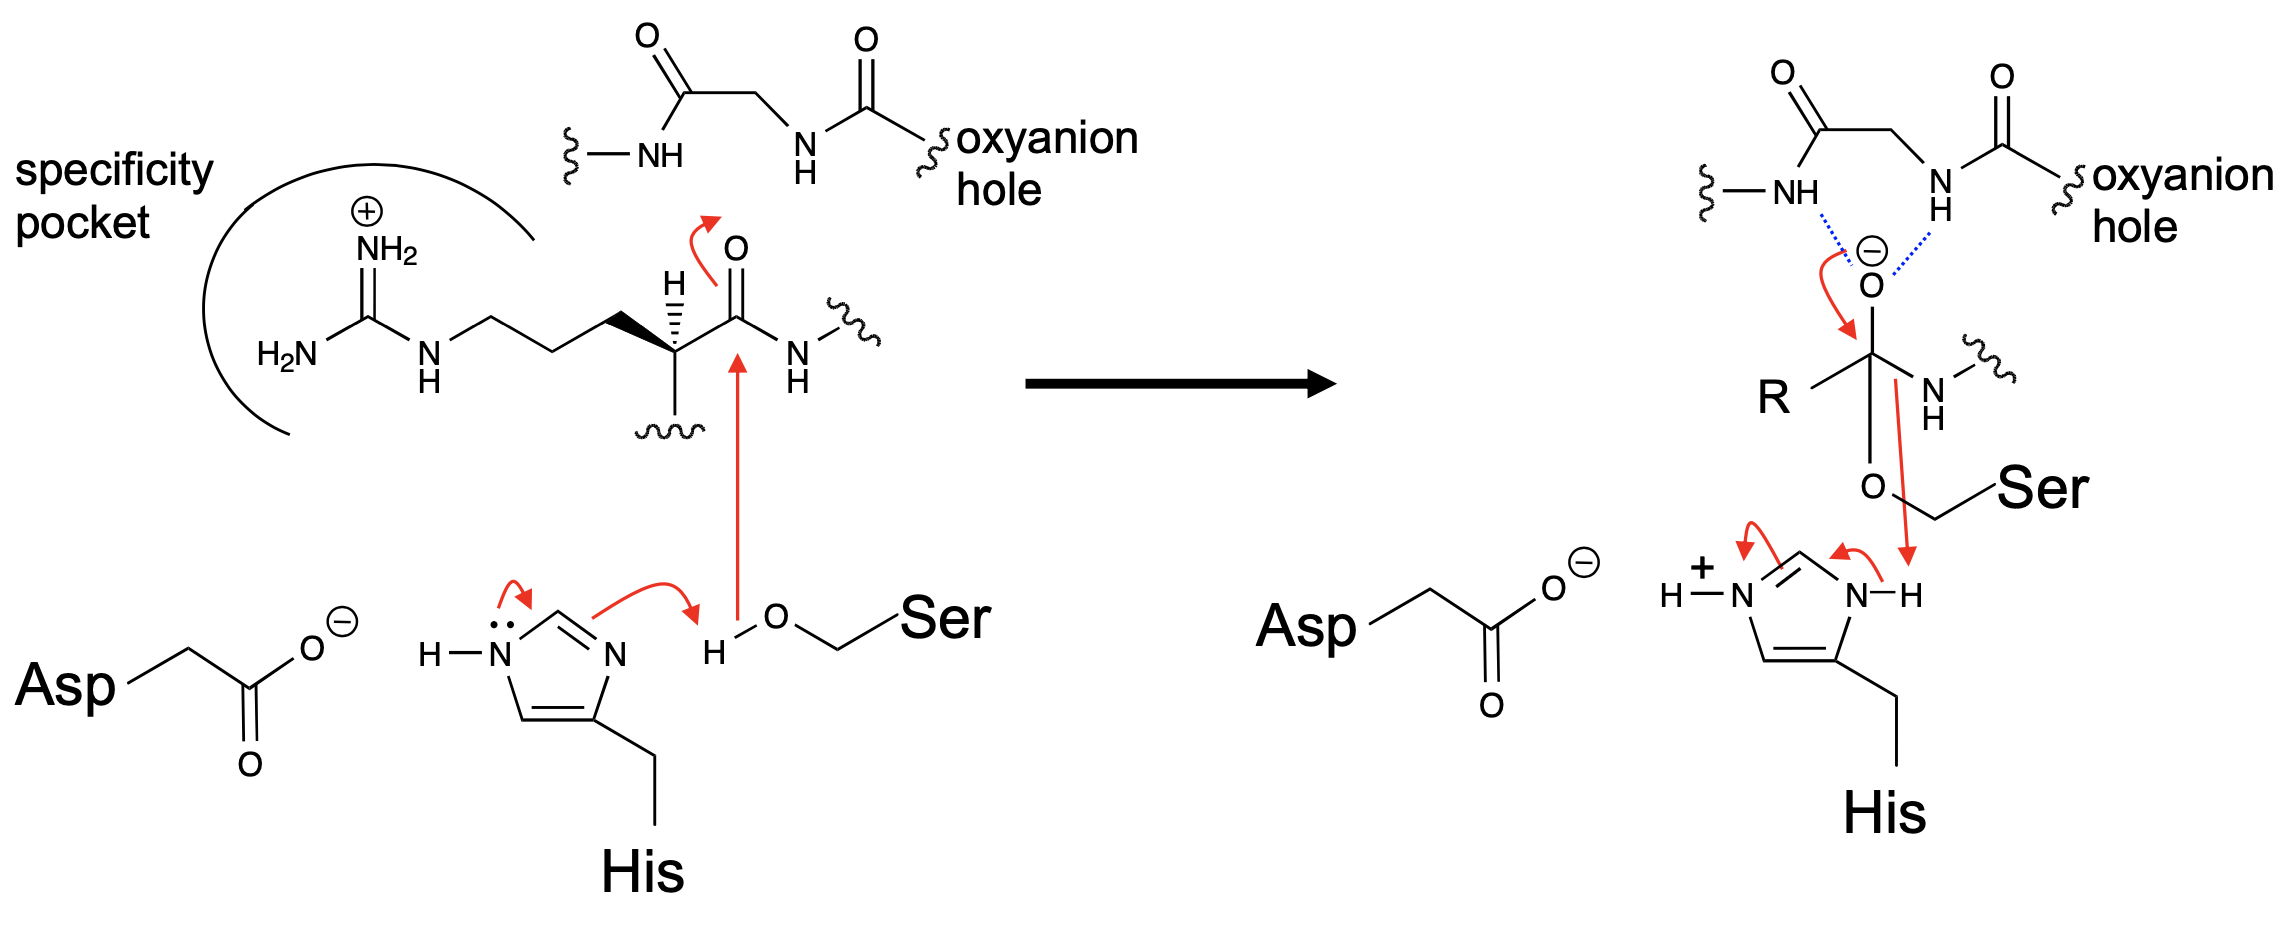
\includegraphics[width=0.8\linewidth]{../ExtFiles/serineProteasea.png}
            \caption{Step 1.}
            \label{fig:serineProteasea}
        \end{subfigure}\\[2em]
        \begin{subfigure}[b]{\linewidth}
            \centering
            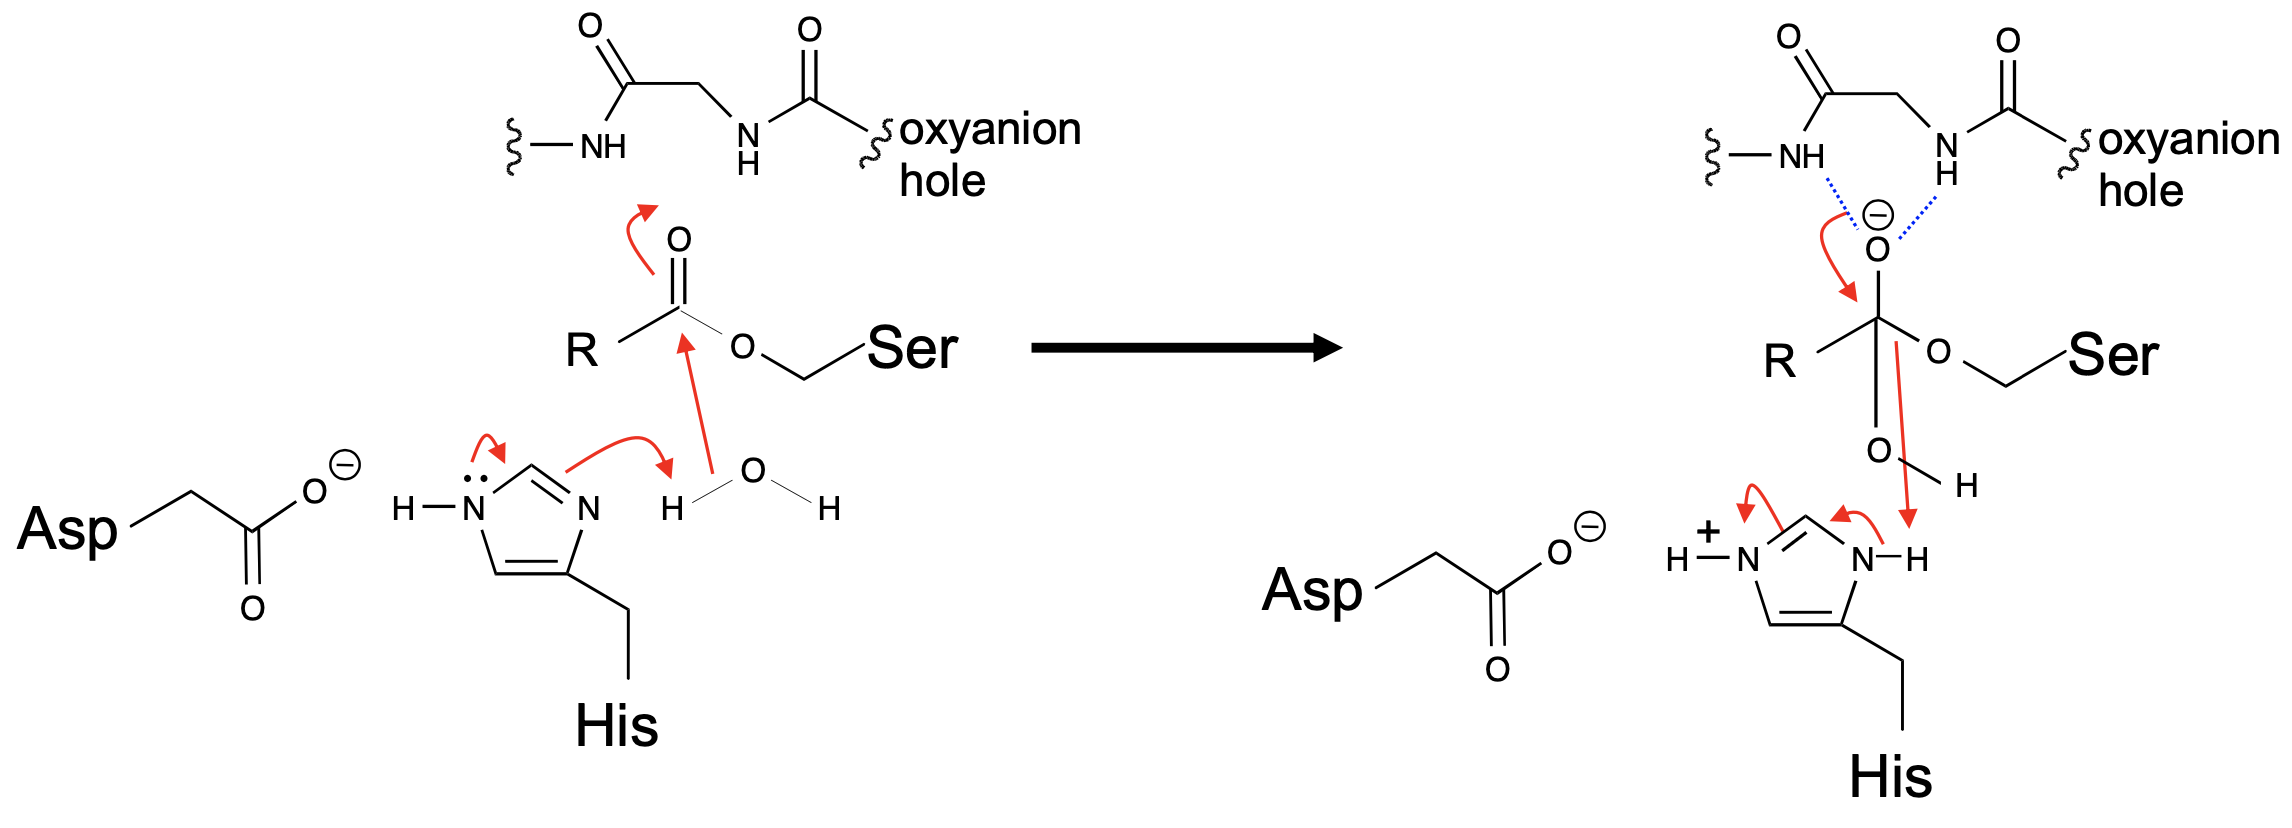
\includegraphics[width=0.8\linewidth]{../ExtFiles/serineProteaseb.png}
            \caption{Step 2.}
            \label{fig:serineProteaseb}
        \end{subfigure}
        \caption{Serine protease.}
        \label{fig:serineProtease}
    \end{figure}
    \begin{itemize}
        \item There is either 1-step or 2-step protease catalysis.
        \begin{itemize}
            \item In 1-step, an acidic side chain (e.g., D, E, or a metal ion [perhaps bound to N or Q]) activates a water molecule to attack the peptide bond.
            \item In 2-step, a nucleophilic side chain (e.g., C, S, or T) splits the peptide bond and then water comes in to break off the side chain from the carbonyl derivative.
        \end{itemize}
        \item Serine protease is a classic example of a protein participating in catalysis covalently; a good example in protein engineering, where it can be developed into a ligase.
        \item Serine protease has a catalytic triad within the active site.
        \begin{itemize}
            \item Histidine (good for its proton shuffle ability) deprotonates serine protease.
            \item The now positively charged histidine is stabilized by the negatively charged aspartate (though protonation/deprotonation does not occur).
            \item Now that serine has been deprotonated, it is an excellent nucleophile and can attack the peptide amide via nucleophilic acyl substitution. The departing amine grabs an extra proton back from histadine.
            \item In step 2, we have another histadine-involved deprotonation to start, but this time of water.
            \item The lone hydroxyl group then attacks the serine-bonded amino acid's carbonyl group again, doing a transesterification nucleophilic acyl substitution, and serine regenerates itself from the histadine proton.
        \end{itemize}
        \item Note that most serine proteases come with a specificity pocket that recognizes one specific type of amino acid at which we want to cleave the peptide bond.
        \item Serine proteases are quite important.
        \item Penicillin (the antibiotic) works by inhibiting a kind of serine protease in bacteria (a transpeptidase used to build the cell wall) that's not found in humans. This makes it so that bacteria cannot construct their cell walls.
    \end{itemize}
    \item Lecture summary.
    \begin{itemize}
        \item 20 natural amino acids offer different features.
        \item Post-translational modifications and rearrangements expand the functional repertoire of proteins.
        \item Protein structure is determined by the nature of the amide bond and by at least four noncovalent interactions (and disulfide bonds).
        \item Natural protein structures are highly modular (helix, sheet, loop; motif; domain; protein) and typically satisfy several constraints.
        \item Side chain structure determine accessible conformational space at each peptide bond.
        \item A subset of proteins serve as catalysts for chemical conversions by lowering the activation barrier.
    \end{itemize}
\end{itemize}




\end{document}